\documentclass[draft]{agujournal2018}
\usepackage{apacite}
\usepackage{url} %this package should fix any errors with URLs in refs.
\usepackage{lineno}
\linenumbers
\draftfalse
\journalname{JGR: Earth Surface}

%% you probably have to kill these custom commands later %% 
\newcommand\be{\begin{equation}} % shortcut to start eq envs 
\newcommand\ee{\end{equation}}   % shortcut to end eq envs
\usepackage{amsmath,amssymb,amsfonts,amsthm}
\usepackage{comment}
\usepackage{wrapfig}
\usepackage{lipsum}
\usepackage{booktabs} % for wrapping text around tabulars in accord with
% https://tex.stackexchange.com/questions/49300/wrap-text-around-a-tabular

\begin{document}

\title{Stochastic birth-death model of heavy-tailed fluvial sediment resting times}
\authors{James K. Pierce\affil{1}\thanks{Vancouver, British Columbia, Canada}, and Marwan A. Hassan\affil{1}\thanks{Vancouver, British Columbia, Canada}}
\affiliation{1}{Department of Geography, University of British Columbia}
\correspondingauthor{James K. Pierce}{kpierce@alumni.ubc.ca}

\begin{keypoints}
\item We model fluvial bedload activity and local bed elevation as a two-species stochastic birth-death process.
\item The resulting timescales of sediment storage by burial lie on heavy-tailed power-law distributions. 
\item Our model describes a virtual velocity of tracer particles may decline indefinitely toward zero as their lifetime in the channel increases.
\end{keypoints}

\begin{abstract}
A consensus has formed that fluvial sediment expresses heavy-tailed statistical distributions of resting times due to the effect of sediment burial on its mobility, and this has key implications for the diffusion of sediment and evacuation of contaminants from river channels.
Owing to observational difficulties, only a handful of experiments have resolved these heavy-tailed resting time distributions, and there have been few theoretical attempts to build understanding.
These studies do not agree on the form or properties of resting time distributions.
In this work, we develop a new stochastic theory which jointly describes bedload transport and bed elevation changes, and we derive resting time distributions for sediment undergoing burial in terms of the joint dynamics.
Our theory corroborates a subset of existing experimental and theoretical work, expressing resting time distributions for sediment undergoing burial with heavy power-law tails, implying super-diffusion of bedload.
Our key finding is that the largest bedload resting times are controlled not only by the erosion and deposition rates, as suggested by earlier studies, but also by the scaling of erosion and deposition rates with local changes in bed elevation.
\end{abstract} 

\section{Introduction}

Classical theories of bedload transport in rivers relate the bulk downstream flux of sediment to characteristics of the hydraulic forcing \citep[e.g.][]{Yalin1972}.
Although bulk fluxes are often described using deterministic models \citep[e.g.]{Wilcock2003}, the individual motions constituting them are more like a random walk, being an alternating sequence of motions and rests which are best characterized statistically \citep[e.g.][]{Einstein1937}.
The statistical properties of individual motions generate differences in the virtual velocities of grains, and these differences imply diffusion, or a spreading out of grains as they transport downstream \citep{Einstein1937, Yano1969, Nakagawa1976}.
Diffusion is important in applications where the downstream transport of only a subset of grains is of interest, as in contaminant evacuation \citep{Malmon2005}, river restoration \citep{Gaeuman2017}, and bed texture adjustment \citep{Hassan2017}, highlighting bedload diffusion as an important topic for study.
 
In the classic diffusion problems, such as the Brownian motion of pollen grains in water \citep[e.g.][]{Einstein1905}, the variance of particle positions $\sigma_x^2$ scales with time $t$ as $\sigma_x^2 \propto t$, a rate of spreading called Fickian or normal diffusion.
Bedload diffusion is more nuanced.
The nature of bedload diffusion is controlled by the probability distributions of step length and resting time.
If either of these distributions has a heavy-tail, the diffusion is called anomalous instead of normal. 
A heavy-tailed step length or resting time distribution has an exceedance distribution $P(X>x) \sim x^{-\alpha}$ with tail parameter $\alpha < 2$.
Anomalous diffusion is characterized by a non-linear scaling of the variance of particle position with time, as in $\sigma_x^2 \propto t^\gamma$ with $\gamma\neq 1$.
In this expression, $\gamma <1$ is called sub-diffusion and $\gamma > 1$ is called super-diffusion.
In a strongly assymmetric random walk as in bedload transport, heavy-tailed step length distributions imply super-diffusion, while heavy-tailed resting time distributions imply either super or sub-diffusion depending on the value of the tail parameter $\alpha$ \citep{Weeks1998}.

A consensus has formed that step lengths in gravel-bed rivers are thin-tailed \citep{Hassan2013, Bradley2017} while bedload diffusion can be anomalous \citep{Nikora2002, Bradley2010, Martin2012, Zhang2012, Phillips2013, Fan2017}, suggesting heavy-tailed resting times are the source of anomalous diffusion \citep{Martin2012, Bradley2017}.
This perspective highlights the mechanism of heavy-tailed resting times as an important consideration.
A dominant hypothesis is that heavy-tailed resting times stem from sediment burial \citep[e.g.][]{Voepel2013, Martin2014, Bradley2017}.
Conceptually, when grains rest on the bed surface, material transported from upstream can deposit over top of them, burying them away from the flow and preventing their entrainment until the overlying material is removed, increasing sediment resting times and imparting a heavy tail to the distribution.

Although a handful of field studies have resolved heavy-tailed resting times \citep{Voepel2013, Olinde2015, Pretzlav2016, Bradley2017}, these do not resolve sediment burial and exhumation during floods, so they cannot discern whether burial is the mechanism generating heavy-tailed resting times.
To our knowledge, only \citet{Voepel2013} and \citet{Martin2014} have provided direct support for the hypothesis that burial generates heavy-tailed resting times, although details of these works are inconsistent with one another.
\citet{Martin2014} performed experiments in a narrow flume configured so grains formed a single layer in the cross-stream direction, providing direct resolution of sediment burial.
Across a range of flow conditions, they obtained heavy-tailed power-law resting time distributions with a tail parameter $\alpha \approx 1$ which they directly attributed to sediment burial.
Different flow conditions shifted the resting time above which the asymptotic power-law scaling applied, but did not obviously change the value of $\alpha$.
Using a bed activity timescale related to the rate of entrainment or deposition events, they managed to partially collapse their experimental distributions. 

The theoretical component of the \citet{Martin2014} work is similar to that of \citet{Voepel2013}.
Both of these models treat local bed elevations as a bounded random walk, where the bed elevation steps randomly up or down with some probability, although they differ in that \citet{Voepel2013} introduces upper and lower bounds to the local bed elevation with hard reflecting barriers, while \citet{Martin2014} introduces them with a softer mean-reverting tendency.
Both of these models are formally similar to classic stochastic theories of the resting times of sand grains on a duned bed \citep[e.g.][]{Yang1971, Nakagawa1980}.
Within these models, the timescales of sediment burial are interpreted as the return time from above in the bed elevation time-series.
From their assumptions, \citet{Voepel2013} conclude the resting time distribution should be a so-called tempered Pareto distribution, with an initial power-law decay which transitions to take on a thin-tailed exponential scaling \citep[e.g.][]{}, and they note agreement between their predictions and the field data of \citet{Habersack2001}.
In contrast, \citet{Martin2014} predicted a heavy-tailed power-law distribution of resting times which does not temper to an exponential distribution, and they successfully calibrated this model to their extensive set of flume experiments.

We believe the differences between these models deserve further theoretical clarification, and we note that although bedload transport is the underlying process driving changes in bed elevation, neither of these models directly incorporate it.
In this paper, we leverage existing knowledge about bedload transport to study the resting times of coarse sediment under burial.
We extend the stochastic bedload transport theory of \citet{Ancey2008} to include bed elevation changes, and we use this model to compute the resting time distribution for sediment undergoing burial.
From this theory, we 



\section{Theory}

We define a control volume of downstream length $\Delta x$ which contains some number $n$ of moving particles within the water flow and some number $m$ of stationary particles composing the bed at some instant.
For simplicity we consider that all particles are approximately spherical with the same diameter $2a$, so that their mobility and packing characteristics are similar from one particle to the next.
Within the control volume, we follow \citet{Ancey2008} and prescribe events which can occur from one instant to the next to modify the populations $n$ and $m$, and we characterize these events using probabilities per unit time, or rates.
These are: (1) migration of a moving particle into the control volume from upstream; (2) the entrainment of a stationary particle into motion; (3) the deposition of a moving particle into rest; and (4) the migration of a moving particle out of the control volume to downstream.
We assume the time intervals between transitions of any kind are exponentially distributed in accord with the Markov hypothesis, equivalent to the assumption that the current transition rates are independent of their history \citep[e.g.][]{Cox1965}.
These concepts are depicted in figure \ref{fig:concept}. 

If the mean number of particles at rest is $m_0$ and the particles have a packing fraction $\phi$, the deviation from the mean bed elevation given a population $m$ of particles at rest within the control volume is
\be z(m) = \frac{\pi a^2}{\phi \Delta x}(m-m_0) = z_1(m-m_0). \label{eq:ele}\ee
The constant $z_1 = \pi a^2/(\phi\Delta x)$ is an important scale of the problem. 
$z_1$ is the magnitude of bed elevation change (in an average sense across the control volume) associated with the addition or removal of a single particle. 
Following \citet{Ancey2008} almost verbatim we write the probabilities associated with each transition in a small time increment $dt$ as 
\begin{align}
 R_{MI}(n+1,m| n, m) &= \nu + O(dt) & \text{migration in},\\
 R_E(n+1,m-1| n,m)  &= \lambda(m) + \mu(m) n + O(dt) & \text{entrainment},  \\
 R_D(n-1,m+1|n,m) &= \sigma(m) n + O(dt) & \text{deposition},\\
 R_{MO}(n-1,m+1|n,m) &= \gamma n + O(dt) & \text{migration out},
\end{align}
but we modify these equations by introducing an $m$ dependence -- through the local bed elevation $z(m)$-- into the entrainment and deposition rates. 
In writing these relations we have used Landau's big $O$ notation to indicate additional terms of order of $dt$ or smaller.

\begin{figure}
  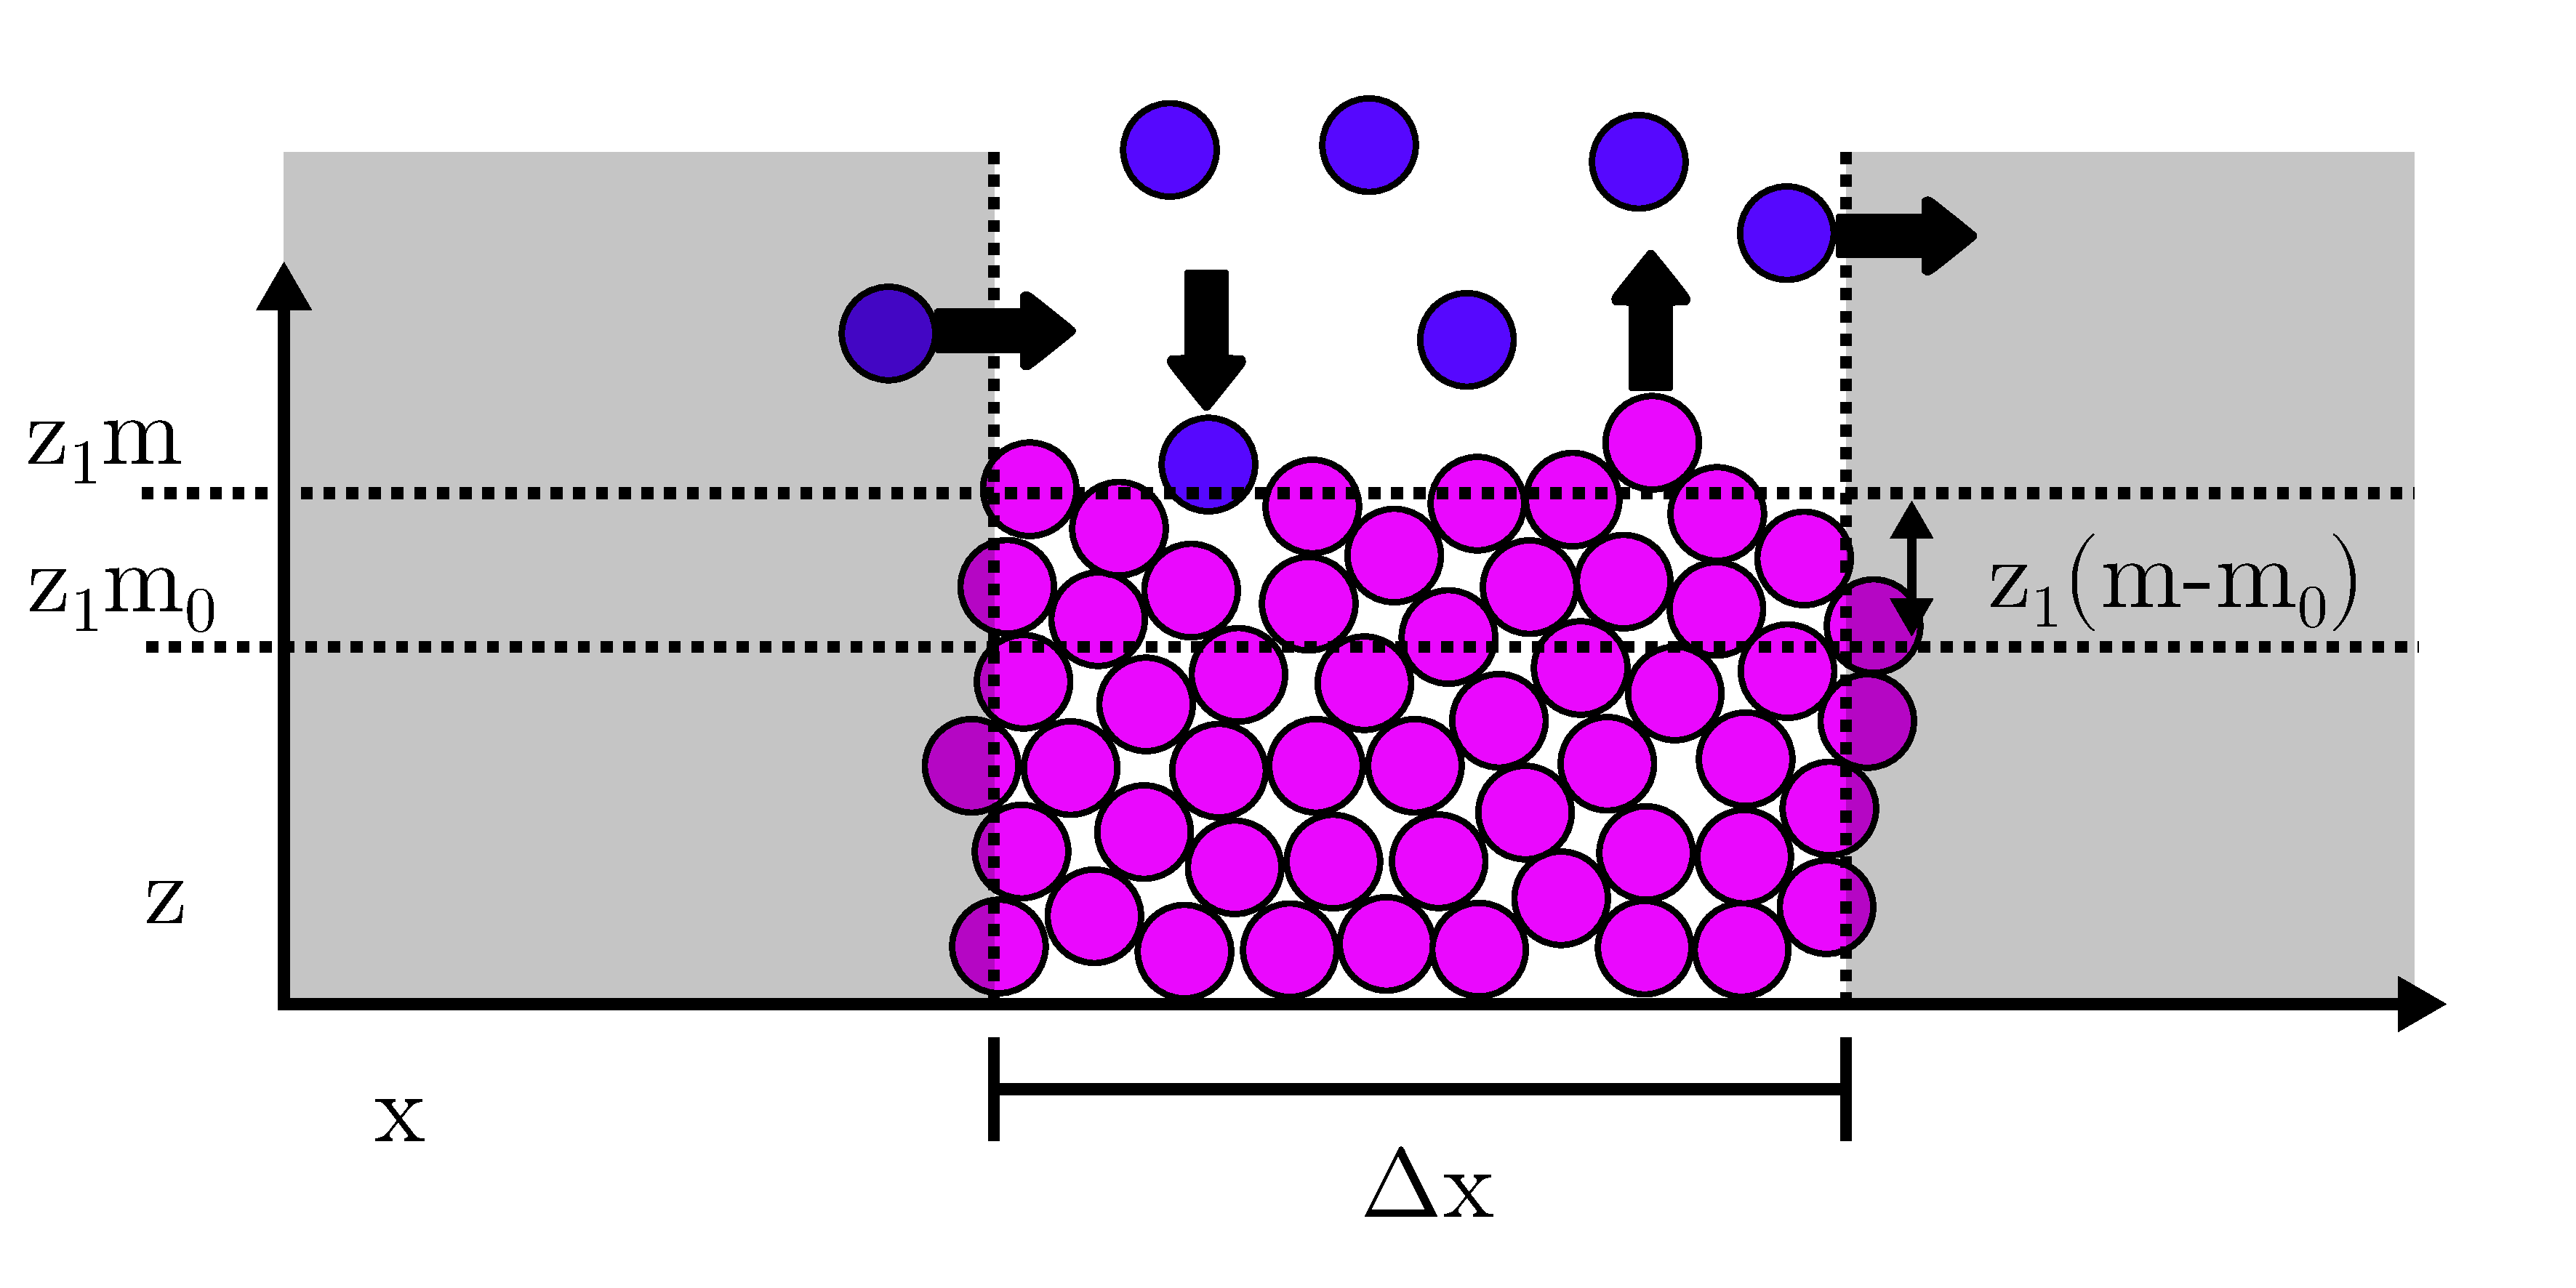
\includegraphics[width=\linewidth,keepaspectratio]{./figures/concept.pdf}
  \caption{The conceptual picture of a control volume containing $n$ moving particles and $m$ resting particles. Migration in, entrainment, deposition, and migration out are represented by arrows, and the probability distribution of bed elevations is illustrated.}
  \label{fig:concept}
\vspace{-1.0cm}
\end{figure}

When entrainment or deposition occurs, they change the local bed elevation which is known to modify subsequent probabilities of entrainment and deposition in negative feedback \citep{Sawai1987, Wong2007}.
\citet{Wong2007} concluded from their experiments that bed elevation changes induce an exponential variation in entrainment and deposition probabilities, while \citet{Sawai1987} concluded from his own experiments that the variation is linear -- a trend also assummed by \citet{Martin2014}.
For simplicity, we incorporate the scaling of \citet{Sawai1987} and \citet{Martin2014}, and we note its equivalence to the \citet{Wong2007} scaling when bed elevation changes are small.
These trends can be incorporated into the entrainment and deposition rates as $\chi(m) = \chi_0(1\pm z_1 z(m)/(2l)^2)$, where $\chi = \lambda, \mu, \sigma$, and entrainment parameters take the plus sign while the deposition parameter takes the minus, so that entrainment is accentuated when $z(m)>0$ and deposition is accentuated when $z(m)<0$. 
With these substitutions, the entrainment and deposition rates become:
\begin{align}
R_E(n+1,m-1| n,m)  &= (\lambda_0 + \mu_0 n)(1 + z_1z(m)/(2l)^2) + O(dt),\\
R_D(n-1,m+1| n,m) &= \sigma_0 (1-z_1z(m)/(2l)^2)n + O(dt).
\end{align} 
At $z(m)=0$, these reduce to the transition rates of the \citet{Ancey2008} theory.
Away from this elevation, entrainment and deposition are alternatively suppressed and accentuated, depending on the sign of $z(m)$, introducing a mean-reverting character to bed elevations similar to the \citet{Martin2014} theory. 
In these equations, $l$ is a length scale of bed elevation change at which the entrainment and deposition rates are significantly affected, and the ratio $z_1/l$ controls the sensitivity of these feedbacks to the addition or removal of a single particle.
The feedbacks between bed elevation changes and entrainment and deposition are strong if $z_1/l$ is large, and they're weak if $z_1/l$ is small.
These equations reflect the trend that entrainment is more likely from regions of exposure, while deposition is more likely in regions of shelter \citep[e.g.][]{Wong2007}.

Within our model, a transition from a state $n,m$ to a state $n',m'$ occurs in a small increment $dt$ of time with probability
\begin{multline}
R(n',m'|n,m) = R_{MI}(n',m'| n, m)\delta_{n',n+1}\delta_{m',m} \\ + R_E(n',m'|n,m)\delta_{n',n+1}\delta_{m',m-1} \\+ R_D(n',m'|n,m)\delta_{n',n-1}\delta_{m',m+1}\\ + R_E(n',m'|n,m)\delta_{n',n-1}\delta_{m',m+1}  + O(dt), 
\end{multline}
being zero for all transitions except the allowed four: (1) migration in, (2) entrainment, (3) deposition, and (4) migration out.
The forward Kolmogorov equation $P(n,m; t+dt) = \sum_{n',m'}R(n',m'|n,m)P(n,m; t)$ describing the flow of probability at the state $n,m$ between times $t$ and $t+dt$ is
\begin{multline}
 \frac{\partial P}{\partial t}(n,m;t) =  
\nu P(n-1,m;t) + 
\{\lambda(m+1) + [n-1]\mu(m+1)\}P(n-1,m+1;t)\\ + 
[n+1]\sigma(m-1)P(n+1,m-1;t) + 
[n+1]\gamma P(n+1,m;t) \\- 
\{ \nu + \lambda(m) + n\mu(m) + n\sigma(m) + n \gamma \}P(n,m;t)
 \label{eq:master}
\end{multline} 
in the $dt \rightarrow 0$ limit \citep{Cox1965,Gillespie1992}.
This is the master equation for the probability distribution $P(n,m;t)$ that there are $n$ moving particles and $m$ stationary particles at time $t$ within the control volume. 
Its solution provides probability distributions for the particle activity, a proxy for the bedload rate \citep[e.g.][]{Ancey2008, Furbish2012}, and the number of resting particles, linked through equation \ref{eq:ele} to the local bed elevation.
This model is a two-species stochastic birth-death theory \citep[e.g.][]{Pielou1977} for the joint dynamics of bedload transport and bed elevations.

\section{Simulations}

Equation \ref{eq:master} does not admit an analytical solution, at least not by the methods applied to similar systems in the population ecology literature \citep[e.g][]{Swift2002}.
In response to this difficulty we pursue a numerical simulation.
Simulation of these birth-death type master equations has been extensively studied for its relevance to chemical physics and population ecology. 
Balancing conceptual simplicity against computational efficiency, we choose the classic Gillespie algorithm \citep{Gillespie1977, Gillespie1992, Gillespie2007}. 
The Gillespie algorithm leverages the defining property of Markov processes that the time interval between any subsequent transitions is exponentially distributed.
When a transition occurs, its type is randomly selected depending on the relative rates of all possibilities.
Accordingly, to step our birth-death process through a single transition, we can select the time to the next transition by drawing a random value from an exponential distribution, then we select the type of transition which occurs by selecting a random value from a uniform distribution. 
After this transition is enacted, i.e., by stepping $n$ and $m$ by the shifts associated with the type of transition which occurred, this two-stage selection is repeated indefinitely to form an exact realization of the stochastic process \citep{Gillespie1977, Gillespie1992, Gillespie2007}.
Computing the joint statistics of $n$ and $m$ from these simulations provides a numerical approximation of equation \ref{eq:master}.

\begin{wraptable}{l}{0.5\textwidth}
\caption{Parameters from \citet{Ancey2008} experiments describing the rates of migration in, entrainment, deposition, and migration out of the control volume when $z(m)=0$. All units are $s^{-1}$ (probability/time).}\label{tab:anceyparams}
\begin{tabular}{cccccc} \\ 
\toprule  
Flow & $\nu$ & $\lambda_0$ & $\mu_0$ & $\sigma_0$ & $\gamma$ \\
\midrule
(a) & 5.45  & 6.59  & 3.74 & 4.67 & 0.77 \\
\midrule
(g) & 7.74  & 8.42  & 4.34 & 4.95 & 0.56 \\
\midrule
(i) & 15.56 & 22.07 & 3.56 & 4.52 & 0.68 \\
\midrule
(l) & 15.52 & 14.64 & 4.32 & 4.77 & 0.48 \\
\midrule
(n) & 15.45 & 24.49 & 3.64 & 4.21 & 0.36 \\
\bottomrule
\end{tabular}
\end{wraptable} 
Using Gillespie's stochastic simulation algorithm, we simulated 5 flow conditions from the \citet{Ancey2008} experiments, prescribing 8 different values of the parameter $l$, ranging from half of the particle radius ($l=a/2$) to 4 particle diameters ($l=8a$) for a total of 40 simulations.
The parameters used for our simulations are taken from the experiments of \citet{Ancey2008} and are summarized in table \ref{tab:anceyparams}.
They are labeled (a), (g), and so on, in order of increasing bedload transport rate. 
Depending on the flow condition, exact stochastic trajectories consistent with equation \ref{eq:master} were simulated for either a $500$ hr or $1,000$ hr duration.
In all simulations, we take the packing fraction $\phi = 0.6$, a typical value for a pile of spheres \citep{Bennett1972}, and set $\Delta x = 22.5cm$ and $a = 0.3 cm$ in accord with the \citet{Ancey2008} experiments.

One simulated realization of our joint stochastic process for bed elevations and bedload transport is depicted in figure \ref{fig:pdfs} (a). 
These realizations determine the joint statistics of $n$ and $m$. 
The bedload transport statistics are depicted for a subset of all simulation conditions in figure \ref{fig:pdfs} (b). 
The \citet{Ancey2008} theory predicts negative binomial distributions for the number of moving particles within the control volume, and the mathematical form of these distributions is apparently not changed by our extension to account for feedbacks between bed elevation changes and entrainment and deposition probabilities.
We obtain an excellent negative binomial fit to the marginal probability distribution of $n$, $P(n) = \sum_m P(n,m,t)$, for all 40 of our simulation results.
However, particle activity statistics, including the mean particle activity and the variance of particle activity, are definitely shifted by the inclusion of differential mobility with bed elevation changes.
Bed elevation changes appear to buffer the magnitude of bedload fluctuations by up to 30 percent, which is an expected effect of the model, since a rapid increase in the bedload rate induced by a series of many entrainments will lower the bed elevation and increase the probability of deposition, buffering the magnitude of the bedload rate increase.

\begin{figure}[t!]
  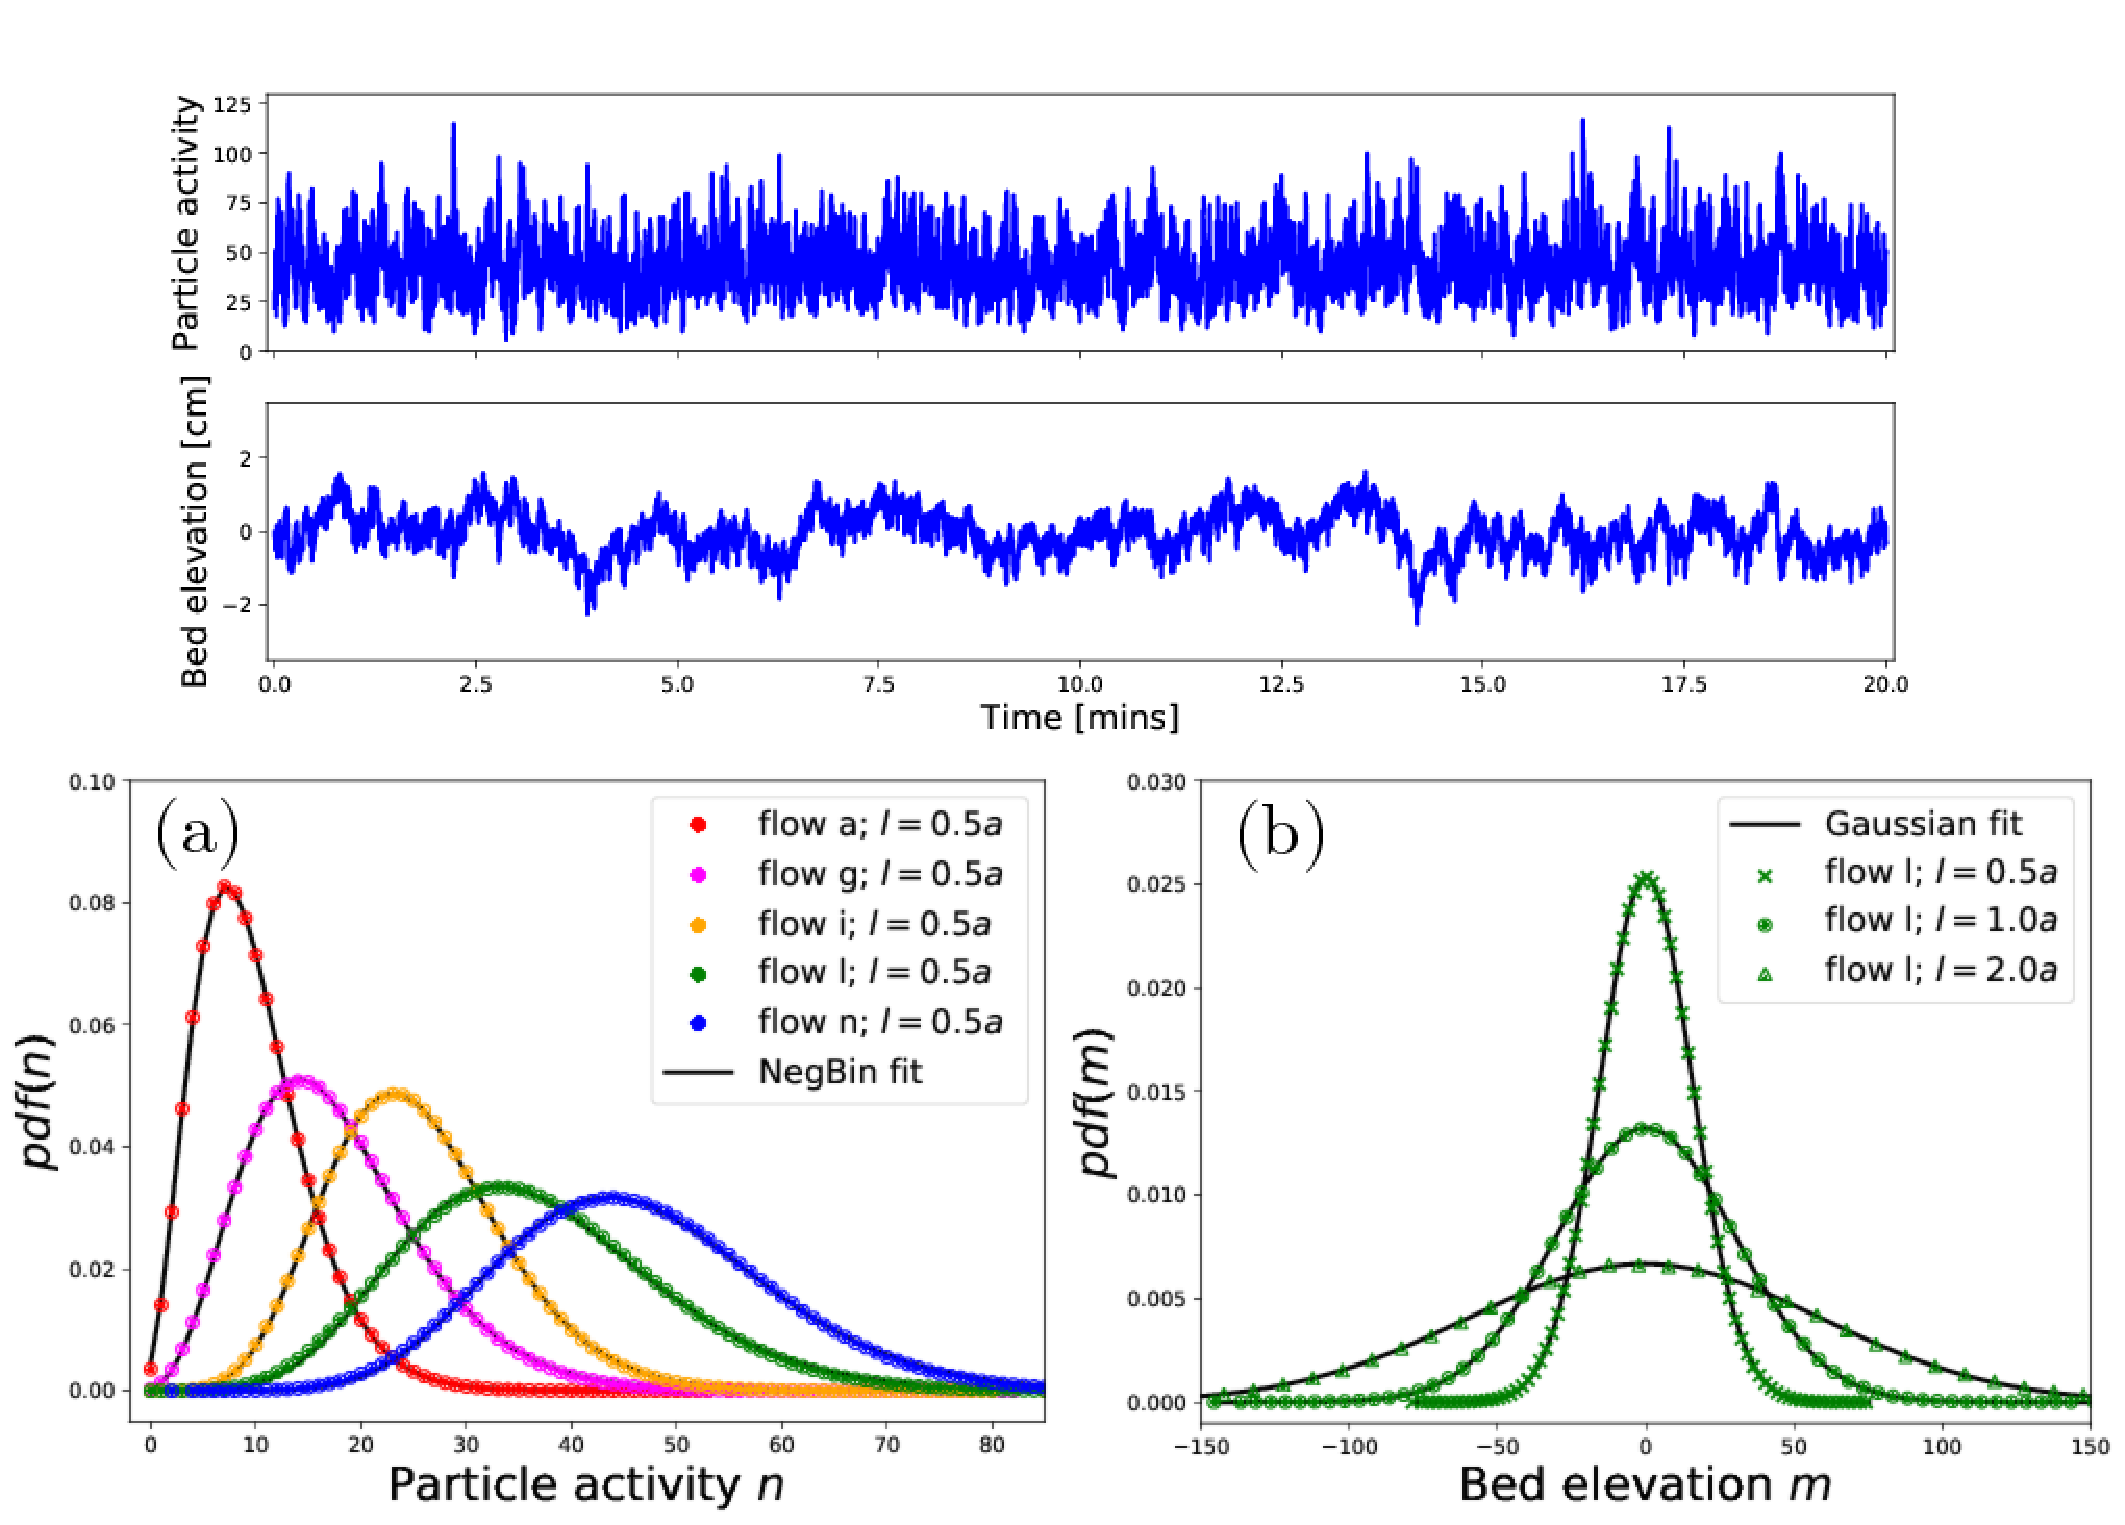
\includegraphics[width=\linewidth,keepaspectratio]{./figures/out2.pdf}
  \caption{Figure (a) depicts timeseries of particle activity and bed elevation over a $20$ minute interval. Figures (b) and (c) display probability distribution functions of bed elevation (equation \ref{eq:ele}) and particle activity for a subset of the simulations. Colors represent flow conditions, while differing line styles represent different values of the differential mobility parameter $l$.}
\vspace{-1.0cm}
  \label{fig:pdfs}
\end{figure}

Our bed elevation timeseries exhibit longer temporal correlations than related bedload activity series, evident in figure \ref{fig:pdfs} (a). 
All 40 of our simulations develop clean unimodal distributions of bed elevations which are fit by Gaussian distributions with excellent correlation, and a subset of these marginal bed elevation pdfs with their Gaussian fits are displayed in figure \ref{fig:pdfs} (c). 
The mean number of particles resting on the bed is $m_0$, corresponding to a relative elevation $z(m_0)=0$. 
The variance of bed elevations is controlled by the differential mobility parameter $l$. 
Apparently, the simulations support the conclusion that $var(m) = (l/z_1)^2$. 
This conclusion is evident in figure \ref{fig:var}, with generally excellent correpsondence between this relationship and the simulation points, with some scatter we attribute to the finite duration of our simulations.

To compute the resting time distribution; at each elevation $m$, we extract the set of all departure times from this elevation, or times at which the bed was at this elevation and a deposition occurred; then we extract the set of all return times to this elevation, or times at which the bed was one increment above this elevation ($m+1$) and an entrainment occurred.
Taking differences between these two time-series returns the set of all return times from above marginal to the elevation $m$, which we binned across a $0.5$s interval to compute the cumulative probabilities of return times at each elevation m, $P(T_r>t|m)$.
Following earlier investigators, we computed the unconditional or over-all rest time distribution as the convolution of these conditional distributions over all bed elevations \citep[e.g.][]{Yang1972, Voepel2013}:
\be P(T_r>t) = \sum_m P(m) P(T_r > t| m), \ee
where $P(m)$ is the pdf of bed elevation like those depicted in figure \ref{fig:pdfs} (b) and the sum is over all bed elevations attained during the simulation. 

\begin{wrapfigure}{r}{0.5\textwidth}
\centering
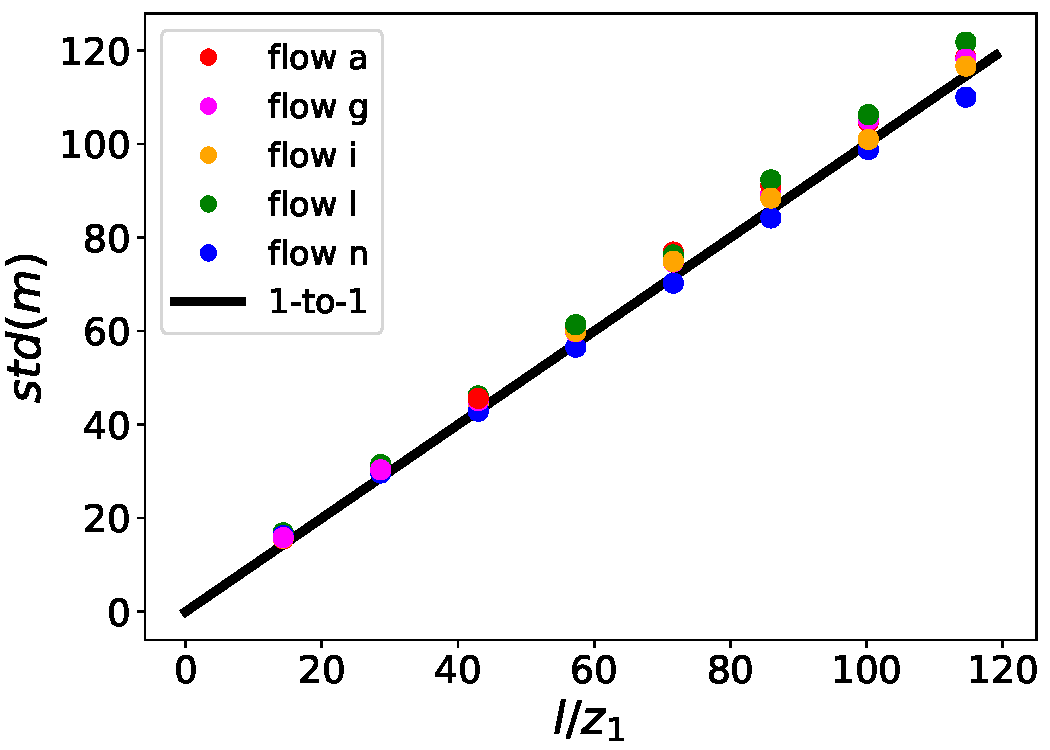
\includegraphics[width=0.5\textwidth,keepaspectratio]{./figures/varm_vs_l.pdf}
\caption{The standard deviation of bed elevation scales one-to-one with the differential mobility parameter $(l/z_1)$, indicating the ratio $l/z_1$ controls the magnitude of bed elevation fluctuations. }
\label{fig:var}
\end{wrapfigure}

This analysis derives unconditional exceedance probabilities of resting times with heavy power-law tails. 
A subset of all of our simulation results are depicted in figure \ref{fig:collapse} (a)-(d). 
Apparently, for suitably long times, the tail parameter $\alpha$ of these resting time distributions is independent of flow conditions or the differential mobility parameter $l$. 
However, the timescale at which particle resting transitions from exponential to power-law scaling shifts with flow conditions and $l$. 
\citet{Martin2014} obtained an approximate collapse at the tails of their experimental resting time distributions using the reciprocal of the rate of entrainment or deposition events occurring. They denoted this rate by $a$, so that their timescale was $1/a$.
Scaling the resting times by $1/a$ provides an incomplete collapse of the tails of our simulated resting time distributions, which may describe the incomplete collapse of the experimental data of \citet{Martin2014}.  
It collapses the tails across flow conditions when $l$ (the standard deviation of bed elevation) is fixed, i.e., it leads to the collapse seen between figures \ref{fig:collapse} (a) and \ref{fig:collapse} (b), but if $l$ (which is the standard deviation of bed elevation) varies with flow, then the power-law scaling of resting times is no longer controlled by $1/a$ alone. 
Instead, we must include a factor representing the differential entrainment and deposition characteristics of grains as the bed elevation changes. 
The timescale which provides universal collapse of the power-law tails of all our simulations is $T_0 = l/(z_1E),$ where $E$ is the entrainment rate.

\begin{figure}[t!] % t for top and ! for force it 
  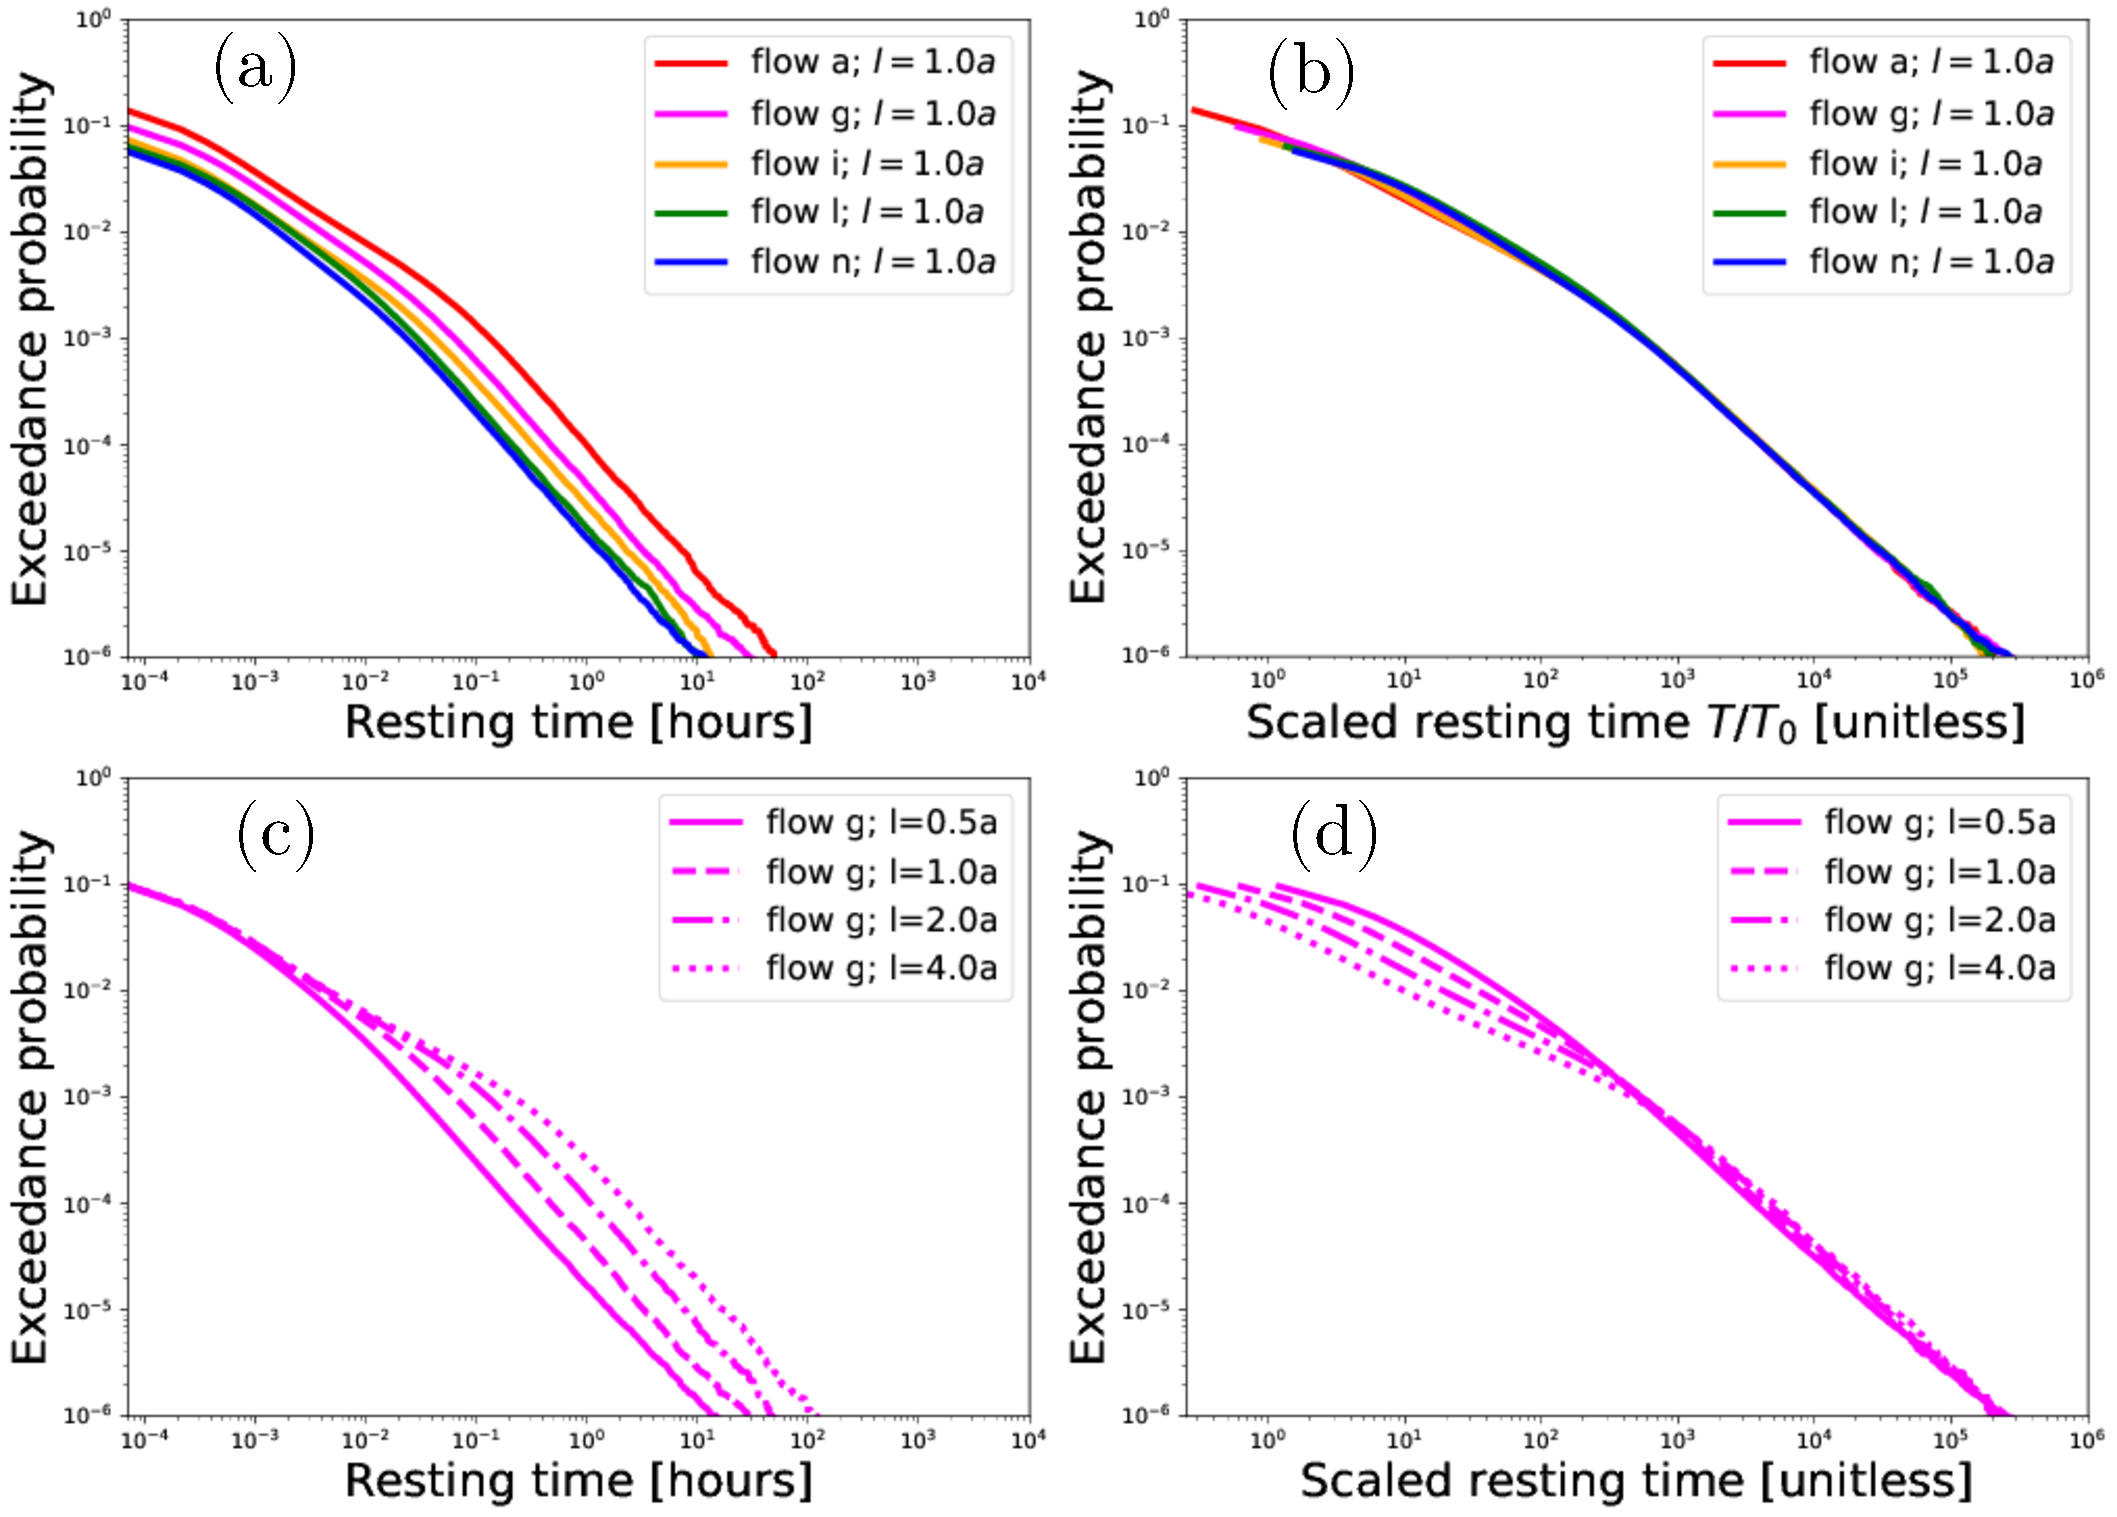
\includegraphics[width=\linewidth,keepaspectratio]{./figures/collapse.pdf}
  \caption{This figure summarizes the resting time exceedance distributions for a subset of all simulations. Part (a) displays resting time distributions for a range of flow conditions at fixed $l$, while part (b) displays the collapse obtained by scaling $T_r$ by $T_0$. The collapse between (a) and (b) is analogous to \citet{Martin2014}, and it is induced by the factor of $1/E$ within $T_0$. Parts (c) and (d) display a similar collapse for a fixed flow condition at variable $l$. In this case, collapse is driven by the factor of $z_1/l$ within $T_0$, and this influence of differential mobility in resting statistics has not to our knowledge been noticed up to now.}
\vspace{-1.0cm}
  \label{fig:collapse}
\end{figure}

We can understand $T_0$ with a physical argument.
According to figure \ref{fig:var}, the typical length scale of bed elevation fluctuations is $l$, and as mentioned the length scale $z_1$ is the magnitude of bed elevation change enacted by the entrainment or deposition of a single particle.  
In equilibrium bedload transport, \citet{Einstein1950} tells us the condition $E=D$ holds: this is a statement of mass conservation. 
Since $E$ represents the mean number of particles removed from the bed in a unit of time, the product $E z_1$ can be interpreted as a representative velocity scale of bed return. 
It is the distance the bed lowers with the removal of a single particle divided by the mean time required to remove it.
Hence we extract our timescale as a key distance scale over a key velocity scale: $T_0 = l/(z_1 E).$ 
Scaling the resting time as $T_r/T_0$ exhibits a consistent power-law tail across all of our simulation results. 

\section{Discussion}

Our theory of bed elevations derives results similar to \citet{Martin2014} using bedload transport as a starting point, and it also provides a statistical characterization of bedload transport.
Our assumptions derive a heavy-tailed power-law distribution of resting times with a tail parameter $\alpha \approx 1$ which displays differences across flow conditions which partially collapse upon scaling by an activity timescale.

However, in extension of the \citet{Martin2014} theory, our model reveals another timescale which fully collapses the power-law tails of the resting time distributions, suggesting a universal power-law should characterize the asymptotic resting times of sediment undergoing burial if the assumptions of our model are correct.
This timescale includes an additional factor characterizing the dependence of entrainment and deposition probabilities on changes in local bed elevations.
We hypothesize this new factor may explain some of the differences between field \citep[e.g.][]{Olinde2015} and laboratory \citep[e.g.][]{Martin2014} observations of resting time distributions, providing additional information to determine whether burial is the dominant mechanism of the heavy-tailed sediment resting times observed in natural channels.

\section{Conclusion}
\begin{comment} 
Bedload diffusion is anomalous because of heavy-tailed sediment resting times \citep{Bradley2017}.
Several theories have shown that heavy-tailed resting times should result from sediment burial \citep{Voepel2013, Martin2014}, and a few experiments have resolved heavy-tailed resting times within natural channels \citep{Olinde2015, Bradley2017}, but these experiments do not support a consensus on the power-law decay, truncation properties, or scaling behavior of the resting time distribution.
Bedload transport and bed elevations vary randomly, so we have pursued a joint stochastic model of these quantities based on a juncture of earlier works \citep{Ancey2008, Martin2014}.
Following the classic literature to interpret burial times as the return time from above in the bed elevation time series \citep{Yang1971, Nakagawa1980}, and including the effect of mobility variation with local bed elevation changes \citep{Sawai1987, Wong2007, Martin2014}, we obtained at a few key conclusions regarding the resting time of sediment undergoing burial.
 
First, particle activities lie on negative binomial distributions, meaning they exhibit relatively wide bedload transport fluctuations. 
This result is essential unchanged from the \citet{Ancey2008} theory, except the moments of the particle activity distribution do shift as a result of bed elevation changes. 
In this work we have chosen to neglect this topic to support a more careful discussion of resting times, but this observation of a negative feedback between bedload fluctuations and bed elevation changes is worth a more careful analysis. 
Second, bed elevations lie on Gaussian distributions, reflecting symmetrical variations in bed elevations, and thin tails which suppress but do not prohibit extreme bed elevation variations.  
Third, and most importantly, the resting time of stationary sediment undergoing burial lies on a heavy-tailed distribution which decays as a power-law with tail parameter $\alpha \approx 1.0$. Our resting time distributions are truncated at a timescale related to the period of observation, and we uncover universal scaling in the power-law decay of these distributions by the timescale $T_0 = l/(z_1E)$.

The timescale $T_0$ is derived from a physical argument: it is the ratio of the representative length scale of bed elevation variations $l$ with a velocity scale of bed elevation changes $z_1 E$. 
Conceptually, $1/E$ is equivalent to the timescale $1/a$ used by \citet{Martin2014} to attain a partial collapse of their resting time distributions across various flow conditions.
Actually, the rate $a$ of entrainment or deposition occurring is $a \approx E+D$, and in equilibrium bedload transport we have $E\approx D$ \citep{Einstein1950}, so $E = a/2$. 
To fully collapse our simulated resting time distributions, the timescale $1/E$ is not sufficient: it collapses across variations in flow but it does not collapse the power-law tails across the concordant variations in the magnitude of bed elevation fluctuations ($l$).
This observation suggests the incomplete collapse of the power-law resting time tails of the \citet{Martin2014} flume experiments, and the appreciable variability of the \citet{Olinde2015} field experiments might be attributed to the differential mobility of bed particles with bed elevation changes, which our model encodes in the ratio $l/z_1$.

In conclusion, we highlight that sediment burial under a region of bed under-going active bedload transport, as we have modeled here, is probably only one mechanism from which natural rivers might express the heavy-tailed sediment burial time distributions which have been observed in tracer experiments \citep{Voepel2013, Olinde2015,Bradley2017}.
The resting time distributions we have simulated, although they have satisfying correspondence with the laboratory experiments of \citet{Martin2014}, where heavy-tailed resting times are verifiably controlled by burial, have limited explanatory power over the excellent field data of \citet{Bradley2017}, which were obtained from a 9 year series of tracer observations.
In natural channels, other mechanisms may induce heavy-tailed resting times of sediment: \citet{Bradley2017} suggested we might look to other stochastic return processes within fluvial channels, such as the return of water levels to tracer particles stranded high on a bar, to gain understanding of sediment resting times.
Similarly, \citet{Malmon2005} suggested sediment residence within floodplains is controlled by the timescales of river channel migration, meaning the resting times of sediment really link to a host of processes from the compounded timescales of individual granular movements, like we have modeled, up to intermediate timescales related to the intermittency of floods, as suggested by \citet{Bradley2017}, all the way up to morphological timescales such as those characterizing channel migration.

Probably, for considerations of contaminant evacuation from gravel bed rivers on typical timescales of ecological relevance (decadal, centennial), a predictive understanding of sediment resting will require the former two processes: sediment burial and water level return. 
In this work, we hope we have created new understanding of the former, uncovering some universal scaling properties.  
The latter topic, which was suggested by Bradley but has not yet been studied, deserves immediate research attention.
According to our model, sediment burial alone is enough to induce fluvial sediment resting time distributions with heavy tails sufficient to drive an arbitrary slowdown of tracer particles or solid contaminants as their period of residence in the channel is increased, and we can state confidently that under idealized conditions when the assumptions of \citet{Einstein1950} are valid, this heavy-tail will decline approximately as $P(T_r) \propto (T_r/T_0)^{-1}$, but we have no idea how these conclusions would be modified by multiple return processes acting in concert, although we hypothesize this could explain the relatively slower decays seen in field data, for example the values of $0.31<\alpha<0.72$ of the \citet{Olinde2015} experiments.
We hope to see subsequent theories deriving resting times from more general channel return processes acting in coordination, and a proliferation of experiments, so we can pin down a mechanistic theory of anomalous diffusion and fluvial contaminant transport.
\end{comment}
\acknowledgments
The computer code used to simulate the presented model is available upon request from the authors.
Marwan A. Hassan is funded by xxx. James K. Pierce is funded by yyy. The authors benefited from conversations with Shawn Chartrand and Conor McDowell. 

\bibliography{biblio}

\end{document}




